\documentclass[10pt]{beamer}
\usetheme[
%%% options passed to the outer theme
%    progressstyle=movCircCnt,   %either fixedCircCnt, movCircCnt, or corner
%    rotationcw,          % change the rotation direction from counter-clockwise to clockwise
%    shownavsym          % show the navigation symbols
  ]{AAUsimple}
  
% If you want to change the colors of the various elements in the theme, edit and uncomment the following lines
% Change the bar and sidebar colors:
%\setbeamercolor{AAUsimple}{fg=red!20,bg=red}
%\setbeamercolor{sidebar}{bg=red!20}
% Change the color of the structural elements:
%\setbeamercolor{structure}{fg=red}
% Change the frame title text color:
%\setbeamercolor{frametitle}{fg=blue}
% Change the normal text color background:
%\setbeamercolor{normal text}{fg=black,bg=gray!10}
% ... and you can of course change a lot more - see the beamer user manual.

\usepackage[utf8]{inputenc}
\usepackage[english]{babel}
\usepackage[T1]{fontenc}
% Or whatever. Note that the encoding and the font should match. If T1
% does not look nice, try deleting the line with the fontenc.
\usepackage{helvet}
\usepackage{tikz}

% colored hyperlinks
\newcommand{\chref}[2]{%
  \href{#1}{{\usebeamercolor[bg]{AAUsimple}#2}}%
}

\title{Private memoirs of a smart meter}

\subtitle{Andrés Molina-Markham, Prashant Shenoy, Kevin Fu, Emmanuel Cecchet, David Irwin}  % could also be a conference name

\date{\today}

\author{
  Bruno Thalmann\\
  \href{mailto:bthalm11@student.aau.dk}{{\tt bthalm11@student.aau.dk}}
}

% - Give the names in the same order as they appear in the paper.
% - Use the \inst{?} command only if the authors have different
%   affiliation. See the beamer manual for an example

\institute[
%  {\includegraphics[scale=0.2]{aau_segl}}\\ %insert a company, department or university logo
  Dept.\ of Computer Science\\
  Aalborg University\\
  Denmark
] % optional - is placed in the bottom of the sidebar on every slide
{% is placed on the bottom of the title page
  Department of Computer Science\\
  Aalborg University\\
  Denmark
  
  %there must be an empty line above this line - otherwise some unwanted space is added between the university and the country (I do not know why;( )
}

% specify a logo on the titlepage (you can specify additional logos an include them in 
% institute command below
\pgfdeclareimage[height=1.5cm]{titlepagelogo}{AAUgraphics/aau_logo_new} % placed on the title page
%\pgfdeclareimage[height=1.5cm]{titlepagelogo2}{AAUgraphics/aau_logo_new} % placed on the title page
\titlegraphic{% is placed on the bottom of the title page
  \pgfuseimage{titlepagelogo}
%  \hspace{1cm}\pgfuseimage{titlepagelogo2}
}

\begin{document}
% the titlepage
{\aauwavesbg%
\begin{frame}[plain,noframenumbering] % the plain option removes the header from the title page
  \titlepage
\end{frame}}
%%%%%%%%%%%%%%%%

%%%%%%%%%%%%%%%%

\section{Context}
\begin{frame}{Context}
  \begin{columns}[T]
    \begin{column}{.5\textwidth}
      \begin{itemize}
        \itemsep1em
  \item Smart meter
  \item Smart appliances and renewable energy
  \item Smart grid
  \item Fine-grained power consumption data
  \item Privacy concerns
  \end{itemize}
    \end{column}
    \begin{column}{.5\textwidth}
      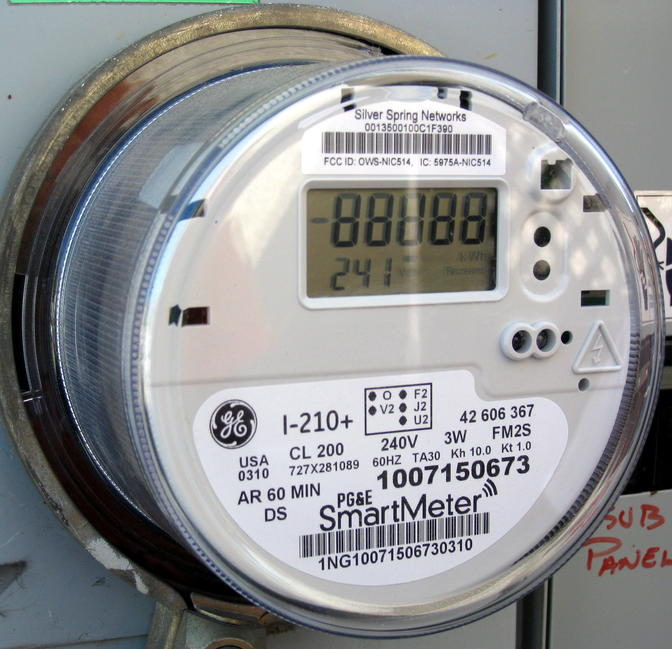
\includegraphics[scale=.5]{graphics/smart-meter.jpg}
    \end{column}
  \end{columns}
\end{frame}

\section{Privacy Concerns}
\begin{frame}{A list of privacy concerns}{}
  \begin{itemize}
    \itemsep2em
  \item Depends on the granularity
  \item Household activities
  \item Number of people home
  \item Information about appliances - by using power signatures
  \item Without prior knowledge?
  \end{itemize}
\end{frame}

\section{Monitored smart meter example}
\begin{frame}{Privacy issues example: Setup}
  \begin{itemize}
    \itemsep2em 
    \item 60 days of power consumption
    \item 3 homes
    \item Power activity journals(min. 3 days)
    \item TED energy monitor
    \item SheevaPlug
    \end{itemize}
\end{frame}

\begin{frame}{Privacy issues example: Setup}
  \begin{center}
  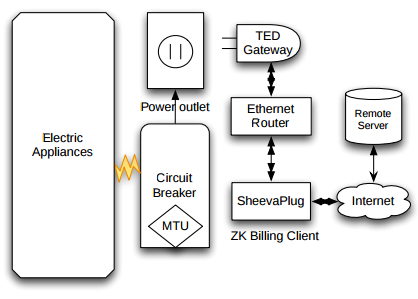
\includegraphics[scale=.5]{graphics/TED_architecture.png}  
  \end{center}
  \begin{itemize}
  \item Outputs: $(t,p)$ for each second
  \end{itemize}
\end{frame}

\begin{frame}{Privacy issues example: Analysis}
  \begin{enumerate}
    \itemsep2em 
  \item Pre-process data using clustering alogrithm
  \item Tag power events with their characteristics
  \item Filter out automated appliances
  \item Map opaque labels to real-life events from external data
  \end{enumerate}
\end{frame}

\begin{frame}{Privacy issues example: Pre-process}
  \begin{enumerate}
  \item Density-based clustering(DBSCAN)
  \item Group tuples by looking at their power pattern and at what time they are measured
  \item Output: power segments
  \end{enumerate}
  \begin{center}
  
\includegraphics[scale=.3]{graphics/weka.png}   
  \end{center}
\end{frame}

\begin{frame}{Privacy issues example: Tag events}
  \begin{itemize}
  \item Each power segments gets labeled
  \item 6 tuple: (segment label, start time, average power, duration, beginning power step, shape label)
  \item Answer questions
  \end{itemize}
\end{frame}

\begin{frame}
            \begin{tikzpicture}[remember picture,overlay]
             \fill [black] (current page.south west) rectangle (current page.north east);
             \node at (current page.center) {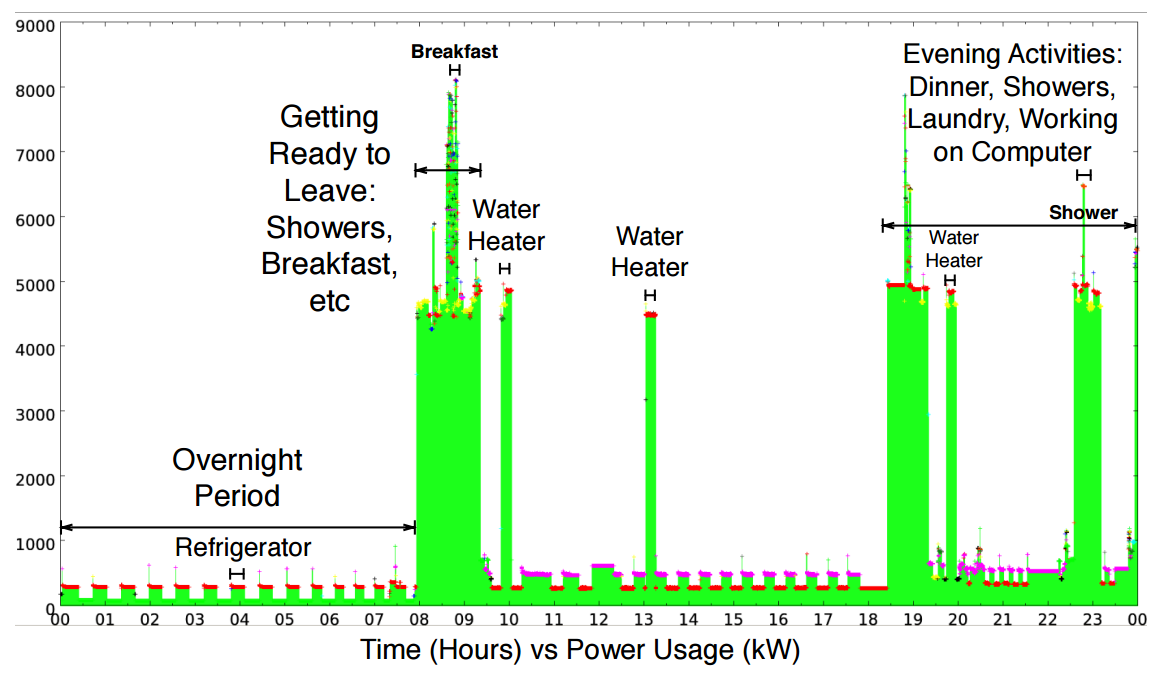
\includegraphics[scale=0.3]{graphics/consumption_one_day.png}};
            \end{tikzpicture}
\end{frame}

\begin{frame}{Privacy issues example: Filtering}
  \begin{itemize}
  \item Filter out automated appliances
  \item Identify automated appliances
  \end{itemize}
\end{frame}

\begin{frame}
  \begin{tikzpicture}[remember picture, overlay]
    \fill [black] (current page.south west) rectangle (current page.north east);
    \node at (current page.center) {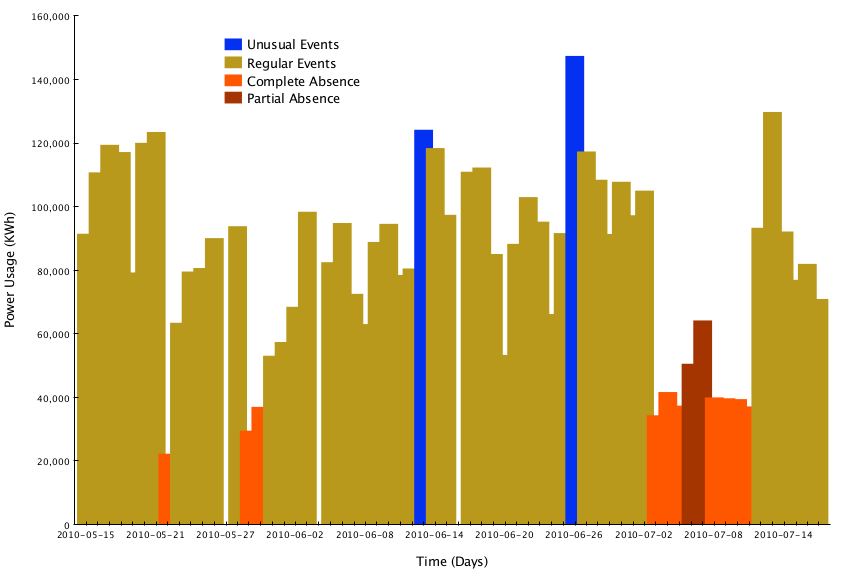
\includegraphics[scale=0.4]{graphics/human_presence.png}};
  \end{tikzpicture}
\end{frame}

\begin{frame}{Privacy issues example: Map events}
  \begin{itemize}
  \item Prior knowledge: Activity journals
  \item Map these to clusters
  \end{itemize}
\end{frame}

\begin{frame}
  \begin{tikzpicture}[remember picture, overlay]
    \fill [black] (current page.south west) rectangle (current page.north east);
    \node at (current page.center) {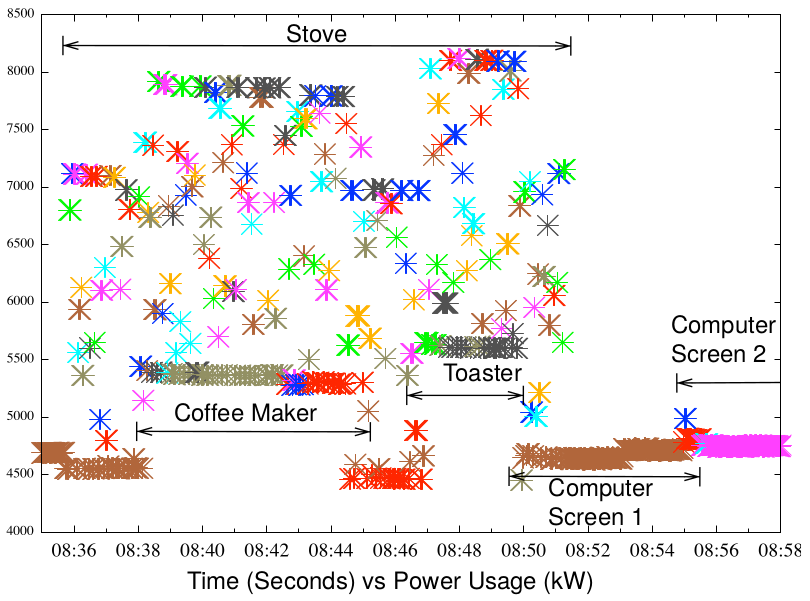
\includegraphics[scale=0.4]{graphics/detailed.png}};
  \end{tikzpicture}
\end{frame}

%%%%%%%%%%%%%%%%

\begin{frame}{Requirements for a privacy enhancing architecture}
  Electric utilities:
  \begin{itemize}
  \item Dynamic pricing
  \item Tamper and energy theft alarms
  \item Power failure and restoration notifications
  \item Demand response for home automation
  \end{itemize}
  Consumer:
  \begin{itemize}
  \item Not revealing when and how energy is being used by a particular household
  \end{itemize}
\end{frame}

\section{Privacy enhancing smart meter architecture}
\begin{frame}{Components}
  Smart meter
  \begin{itemize}
  \item Gather fine grained power readings
  \item (pseudo-random tuple id/tag, timestamp, power usage)
  \item Assumpion: consumers want to tamper with SM
  \end{itemize}
  \pause
  Neighborhood gateways
  \begin{itemize}
  \item Sends data without revealing source: (timestamp, power usage)
  \item Could act as control and storage point
  \item Assumption: Gateways are trusted and communication with SMs and utility servers is safe
  \end{itemize}
  \pause
  Remote utility server
  \begin{itemize}
  \item Collect all the tuples from the gateways
  \item Direct: Zero-Knowledge protocol for billing
  \end{itemize}
\end{frame}


\section{Zero Knowledge Protocol}
\begin{frame}{Zero Knowledge Protocol}
  \begin{itemize}
  \item $prover$, $secret$, $verifier$
  \item Challenge-response authentication
  \item Authentication without telling the $secret$
  \item Interactive verification - sending a series of challenges
  \item Public key identification example
  \end{itemize}
\end{frame}

\section{Commitment Scheme}
\begin{frame}{Commitment scheme}
  Keep something hidden and unchanged until one wants to reveal it.
  \begin{itemize}
  \item Commit phase: Commit some values
  \item Values cannot be changed
  \item Values are hidden to others
  \item Reveal phase: Reveal value and check
  \item Public key identification example continued
  \end{itemize}
\end{frame}

\section{Zero Knowledge Billing Protocol}
\begin{frame}{A zero knowledge billing protocol}
  For each billing cycle:
  \begin{enumerate}
  \item \textbf{Registration} - Commit phase: commit random tags($r_i$) and keys($k_1, \dots, k_m$) where e.g. $m = 10$
  \item \textbf{Tuple gathering} - SM creates tuples: $(r_i, t_i, p_i)$
  \item \textbf{Reconciliation} - Reveal phase: Compute bill and verify
  \end{enumerate}
  Random spot checks
\end{frame}

\begin{frame}{Conclusion}
  \begin{itemize}
  \item Zero knowledge protocols are computationally expensive
  \item Initial results
  \item At a granularity of one minute it takes 5 minutes to verify these measurements
  \end{itemize}
\end{frame}

{\aauwavesbg
\begin{frame}[plain,noframenumbering]
  \finalpage{Questions}
\end{frame}}
%%%%%%%%%%%%%%%%

\end{document}
